% !TEX TS-program = xelatex
% !TEX encoding = UTF-8 Unicode

% Tennessee Technological University
% ENGR1120-021 - GSET - Summer 2023
% Tristan Hill - June 05, 2023
% Module 2 - Variables, Expressions, and Assignment
% Lecture 2 


\documentclass[fleqn]{beamer} % for presentation (has nav buttons at bottom)

\usepackage{/mnt/c/Users/thill/Documents/courses/py_workshop/modules/py_lectures}

\newcommand{\MNUM}{2\hspace{2mm}} % Module number
\newcommand{\TNUM}{---\hspace{2mm}} % Topic number - single topic for now
\newcommand{\moduletitle}{Variables and Assignment} % Titles and Stuff
%\newcommand{\topictitle}{---} 

\newcommand{\sectiontitleI}{Types of Numbers} % More Titles and Stuff
\newcommand{\sectiontitleII}{Variables and Type}
\newcommand{\sectiontitleIII}{Assignment and Memory}
\newcommand{\sectiontitleIV}{A {\it Riddle} }
\newcommand{\sectiontitleV}{A Python Example }

\newcommand{\btVFill}{\vskip0pt plus 1filll}

\setbeamercolor{title in head/foot}{fg=TTUgold} % this needs work...

\title{GSET - Intro to Programming with Python}
\author{Tristan Hill\vspc \hspc Tennessee Technological University \hspc}
\date{Summer 2023}

\begin{document}

\lstset{language=Python,basicstyle=\ttfamily\small,showstringspaces=false}

\frame{\titlepage \center\begin{framed}\Large \textbf{Module \MNUM - \moduletitle}\end{framed} \vspace{5mm}}

% Section 0 - Outline
\frame{
	
	\large \textbf{Module \MNUM - \moduletitle} \vspace{3mm}\\
	
	\begin{itemize}
	
		\item \hyperlink{sectionI}{\sectiontitleI} \vspc % Section I
		\item \hyperlink{sectionII}{\sectiontitleII} \vspc % Section II
		\item \hyperlink{sectionIII}{\sectiontitleIII} \vspc %Section III
		\item \hyperlink{sectionIV}{\sectiontitleIV} \vspc %Section IV	
		\item \hyperlink{sectionV}{\sectiontitleV} \vspc %Section V
	
	\end{itemize}

}


% Section I
\section{\sectiontitleI}

	% Section I - Frame I
	\begin{frame}[label=sectionI] \small
		\frametitle{\sectiontitleI}
		
		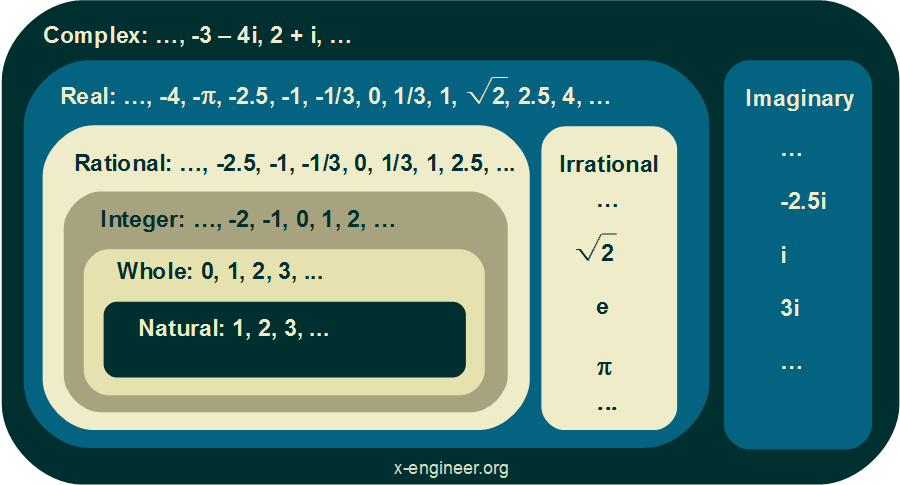
\includegraphics[scale=.35]{types_of_numbers.png} \\
		
				\tiny{Image: \href{https://x-engineer.org/undergraduate-engineering/mathematics/arithmetics/types-of-numbers/}{x-engineer.org}}
	
	\end{frame}

	%\section{\sectiontitleII}	
	
	% Section I - Frame II
	\begin{frame}[label=sectionI] \small
	\frametitle{\sectiontitleI}
	\bigskip
	
	\begin{multicols}{2}
		\begin{tabular}{|r|r|r|} \hline
			Binary 	& Decimal 	& Hexadecimal \\ \hline
			0		& 0			& 0 		\\ \hline	
			1		& 1			& 1 		\\ \hline
			10		& 2			& 2 		\\ \hline
			11		& 3			& 3 		\\ \hline
			100		& 4			& 4 		\\ \hline
			& 5			& 5 		\\ \hline
			& 6			& 6 		\\ \hline
			& 7			& 7 		\\ \hline
			& 8			& 8 		\\ \hline
			& 9			& 9 		\\ \hline
			& 10		& A 		\\ \hline
			& 11		& B 		\\ \hline
		\end{tabular}
		
		\begin{tabular}{|r|r|r|} \hline
			Binary 	& Decimal 	& Hexadecimal \\ \hline
			& 12		& C 		\\ \hline	
			& 13		& D 		\\ \hline
			& 14		& E 		\\ \hline
			& 15		& F 		\\ \hline
			& 16		&  		\\ \hline
			& 17		&  		\\ \hline
			& 18		&  		\\ \hline
			& 19		&  		\\ \hline
			& 20		&  		\\ \hline
			& 21		&  		\\ \hline
			& 22	    &  		\\ \hline
			& 23	    &  		\\ \hline
		\end{tabular}
	\end{multicols}
	
	\btVFill
	\tiny{some reference}		
	
\end{frame}

% Section I - Frame III
\begin{frame} \small
\frametitle{\sectiontitleI}
\bigskip

\begin{multicols}{2}
\begin{tabular}{|r|r|r|} \hline
	Binary 	& Decimal 	& Hex. \\ \hline
	0		& 0			& 0 		\\ \hline	
	1		& 1			& 1 		\\ \hline
	10		& 2			& 2 		\\ \hline
	11		& 3			& 3 		\\ \hline
	100		& 4			& 4 		\\ \hline
	& 			&  		\\ \hline
	& 			&  		\\ \hline
	& 			&  		\\ \hline
	& 			&  		\\ \hline
	& 			&  		\\ \hline
	& 		&  		\\ \hline
	& 		&  		\\ \hline
\end{tabular}

\begin{tabular}{|r|r|r|} \hline
	Binary\hspace{18mm} 	& Decimal 	& Hex. \\ \hline
	0		& 0			& 0 		\\ \hline	
	1		& 1			& 1 		\\ \hline
	10		& 2			& 2 		\\ \hline
	11		& 3			& 3 		\\ \hline
	100		& 4			& 4 		\\ \hline
	& 			&  		\\ \hline
	& 			&  		\\ \hline
	& 			&  		\\ \hline
	& 			&  		\\ \hline
	& 			&  		\\ \hline
	& 		&  		\\ \hline
	& 		&  		\\ \hline
\end{tabular}
\end{multicols}

\btVFill
\tiny{some reference}	
\end{frame}


% Section II
\section{\sectiontitleII}

    % Section II - Frame I
	\begin{frame} \small
		\frametitle{\sectiontitleII}
			
		Types in Python \vspace{5mm}\\
		\renewcommand*{\arraystretch}{1.5}
		\begin{tabular}{|c|c|}\hline			
			Text Type:& str  \\ \hline
			Numeric Types: & int, float, complex \\ \hline
			Sequence Types:& list, tuple, range \\ \hline 	
			Mapping Types:& dict \\ \hline
			Set Types:& set, frozenset\\ \hline
			Boolean Type:& bool \\ \hline
			Binary Types:& bytes, bytearray, memoryview\\ \hline
			None Type: & NoneType\\ \hline	 			
		\end{tabular}
	
	\btVFill
	{\tiny \href{https://www.w3schools.com/python/python_datatypes.asp}{w3schools}}
	\end{frame}


	% Section II - Frame II
	\begin{frame}[label=sectionII,containsverbatim] \small
		\frametitle{\sectiontitleII}

			\begin{lstlisting}
			
	value_A = 100; 
				
	value_B = 25.56j;

	course = "ENGR1220-021-GSET"
			\end{lstlisting}
	
			A variable is a storage container.
			\begin{itemize}
				\item In Python and many other programming languages, each variable has a type determined by the programmer during {\BL Initialization}.
				\item The type can be explicitly used in the initialization for clarity.
			\end{itemize}
	
		\end{frame}

	% Section II - Frame III
	\begin{frame}[label=sectionII,containsverbatim] \small
		\frametitle{\sectiontitleII}
	
	  The type can be explicitly used in the initialization for clarity.
		

		\begin{lstlisting}
			
	value_A = int(100); 
				
	value_B = complex(25.56j);

	course = str("ENGR1220-021-GSET")
			\end{lstlisting}

	
		\end{frame}

	

	% % Section II - Frame III
	% \begin{frame} \small
	% \frametitle{\sectiontitleII}
	
	% Variable type have limited range. \vspace{2mm}\\
	% \renewcommand*{\arraystretch}{1.5}
	% \begin{tabular}{|c|c|c|c|}\hline			
	% 	Type & C++ Syntax & Min Value & Max Value  \\ \hline
	% 	Boolean & bool &  0 (Off) & 1 (On) \\ \hline 	
	% 	Unsigned Integer (4 bytes) & uint &  0 &  \\ \hline
	% 	Signed Integer (4 bytes) & int &   &  \\ \hline
	% 	Unsigned Short Int. (2 bytes) & uint &   &  \\ \hline
	% 	Signed Short Int. (2 bytes) & int &   &  \\ \hline
	% 	Floating Point (4 bytes) & float &  & \\ \hline
	% 	Double Float. (8 Bytes) & double &  &\\ \hline
	% 	Character & char &  &\\ \hline	 			
		
	% \end{tabular}
	
	% \btVFill
	% {\tiny \href{https://www.tutorialspoint.com/cplusplus/cpp_data_types.htm}{Tutorials Point}}
%\end{frame}


% Section III
\section{\sectiontitleIII}


	% Section III - Frame I
	\begin{frame}[label=sectionIII] \small
	\frametitle{\sectiontitleIII}
	
	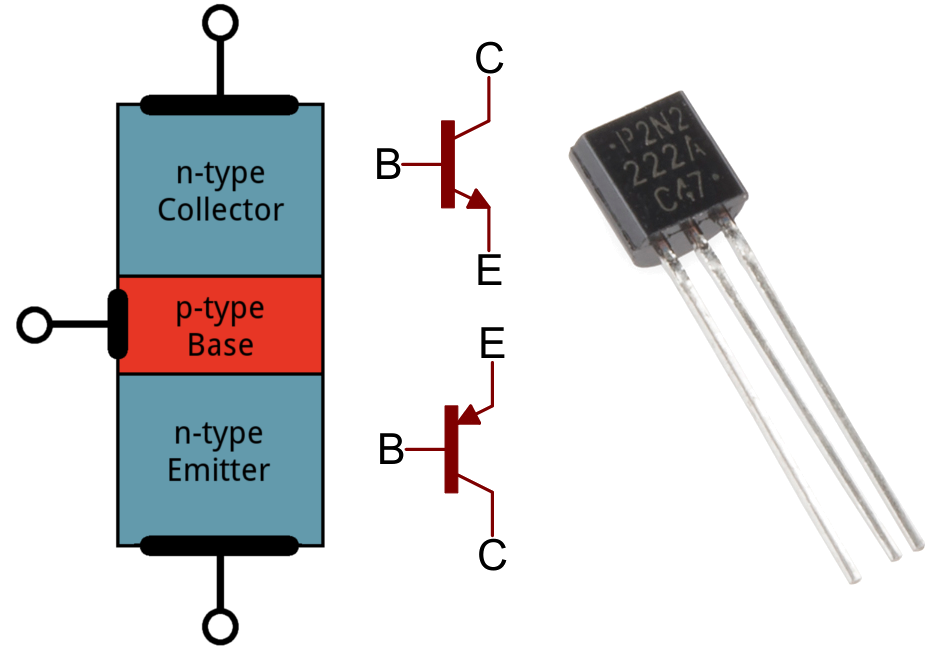
\includegraphics[scale=.15]{transistor_pnp}
	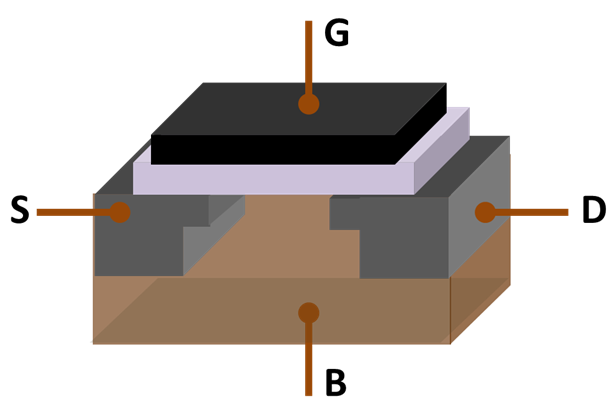
\includegraphics[scale=.25]{MOSFET_Structure.png}
	
	\btVFill
	\href{https://learn.sparkfun.com/tutorials/transistors/all}{Sparkfun - Transistor} \\
	\href{https://en.wikipedia.org/wiki/Transistor}{Wikipedia - Transistor}
	
	\end{frame}

	% Section III - Frame II
	\begin{frame} \small
		\frametitle{\sectiontitleIII}
		
		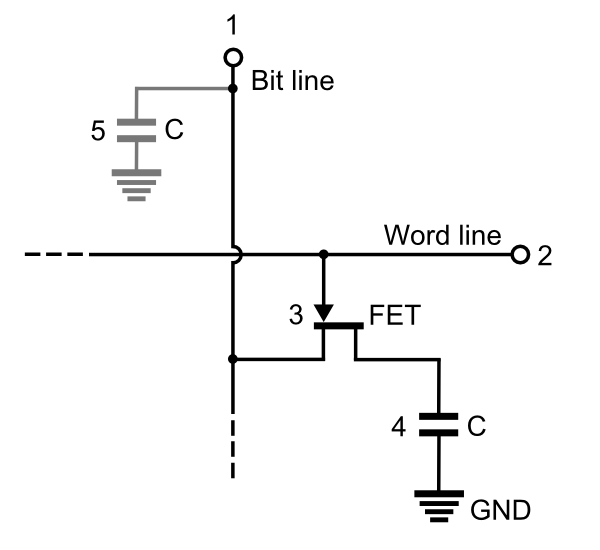
\includegraphics[scale=.20]{DRAM_memcell.png}
		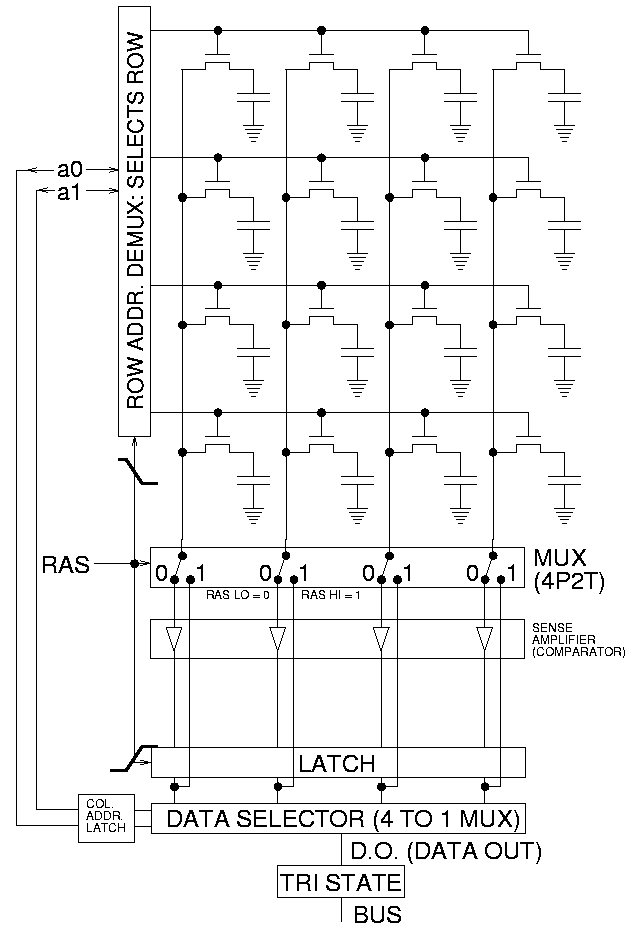
\includegraphics[scale=.10]{Square_array_memcells.png} 
		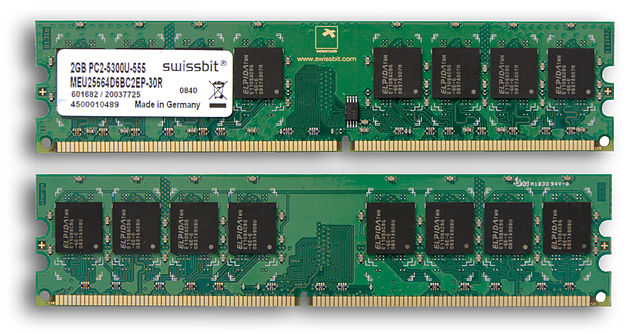
\includegraphics[scale=.50]{ramstick.jpg}
		
		\btVFill
		\href{https://en.wikipedia.org/wiki/Memory_cell_(computing)}{Wikipedia - Memory Cell} \\
		\href{https://en.wikipedia.org/wiki/Semiconductor_memory}{Wikipedia - Semiconductor Memory}
		\href{https://en.wikipedia.org/wiki/Random-access_memory}{Wikipedia - RAM}

	\end{frame}

	% Section III - Frame III
	\begin{frame}[containsverbatim] \small
	\frametitle{\sectiontitleIII}

	\underline{The Assignment Operator} \vspace{5mm} \\

	\begin{lstlisting}
	
		val_A =  53214
	
		val_B = 0
	
	\end{lstlisting}
	
	\begin{itemize}
		\item In Python and many other programming languages, variables are assigned a value using the equals sign. This is called {\BL assignment}.
		\item Typically the value in the variable can be changed, or re-assigned. 
		\item The expression on the right hand side may contain literal values or variables, operators, and functions. 
		
		
	\end{itemize}
	
	
	\end{frame}

		% Section III - Frame III
	\begin{frame}[containsverbatim] \small
	\frametitle{\sectiontitleIII}

	\textbf{Arithmetic Operators in Python} \vspace{5mm} \\

	\renewcommand*{\arraystretch}{1.5}
	\begin{tabular}{|c|c|c|} \hline
		\textbf{Operator}& \textbf{Name}& \textbf{Example} \\ \hline
		+ & Addition& x+y \\ \hline
        - & Subtraction& x-y \\ \hline
        * & Multiplication& x*y \\ \hline
        / & Division& x/y \\ \hline
        \% & Modulus & x\%y \\ \hline
        ** & exponetiation & x**y \\ \hline
        // & floor division& x//y \\ \hline 
	\end{tabular}
	
	
	\end{frame}
	


% Section IV
\section{\sectiontitleIV}	
	% Section IV - Frame I
	\begin{frame}[label=sectionIV] \small
		\frametitle{\sectiontitleIV}    
		
		Question: \vspace{5mm}\\ What is the maximum number of rupees that you can hold in the original {\it Legend of Zelda} video game? 
		\vspace{25mm}
		
		Answer:

	\end{frame}

% Section V
\section{\sectiontitleV}	
	% Section V - Frame I
	\begin{frame}[label=sectionV,containsverbatim] \small
		\frametitle{\sectiontitleV}    
		
		\begin{lstlisting}
# Variables and Assigment - Python - June 6, 2023

val = 56 
	
print("The value is: ",val)
	
\end{lstlisting}

	\end{frame}

\end{document}

